\documentclass[twoside,11pt]{article}
% JMLR first-submission layout. Official, unmodified jmlr2e.sty; 'preprint'
% suppresses publication-only volume/date/editor details not yet assigned.
\usepackage[preprint]{jmlr2e}
\usepackage{amsmath,amssymb,booktabs,multirow,graphicx,array,url}
\usepackage{lastpage}
\newcommand{\PR}{\mathbb{P}}
\newcommand{\EE}{\mathbb{E}}
\newcommand{\Fhat}{\widehat F}
\newcommand{\R}{\mathbb{R}}
\newcommand{\sset}{\mathcal{S}}
\firstpageno{1}
\begin{document}
\title{Coverage Certification Under Population-Mixture Shift from Imperfect Group Proxies}
\author{\name Mohitsing Sanjaysing Patil \\
\addr Independent Researcher\\
Pune, Maharashtra, India\\
\addr rajputmohit0708@gmail.com}
\maketitle
\begin{abstract}%
Prediction intervals calibrated on one population may lose coverage when the proportions of latent subgroups change. The difficulty is sharper when group membership is observed only through a noisy proxy. We study the identifiable setting in which the proxy channel and source and target group proportions are known, while score distributions remain invariant within latent groups. An inverse-mixture identity recovers the target score distribution from observable proxy-stratified distributions. Combining the identity with stratified Dvoretzky--Kiefer--Wolfowitz bounds yields a finite-sample, simultaneous lower confidence envelope for target coverage and a conservative threshold rule. We characterize when that rule becomes uninformative as proxy noise increases and give a non-identifiability example when the proxy channel is singular. In a two-group simulation, pooled calibration achieved 65.5\% mean coverage after a mixture shift; the certified rule achieved 93.5\%, with larger intervals, across 35 repetitions. Controlled resampling from four real-data empirical score populations shows a similar coverage--width trade-off under exactly specified group mixtures and proxy channel; separate ordinary data-split studies expose the cost of plug-in assumptions. The method gives a conditional calibration guarantee under explicit assumptions, not general distribution-free validity under arbitrary shift.
\end{abstract}
\begin{keywords}
conformal prediction, distribution shift, noisy group labels, prediction intervals, finite-sample coverage
\end{keywords}

\section{Introduction}
A seemingly well-calibrated model can become unreliable without its conditional errors changing. A data-collection program may include many observations from an easy subgroup, while deployment encounters mostly harder cases. The old calibration threshold then describes a population that no longer exists. Pooled split conformal prediction is especially transparent about this limitation: its finite-sample guarantee assumes exchangeability between calibration and test data \citep{vovk2005,angelopoulos2023}. Population-mixture shift breaks that relationship even when the predictive model remains fixed.

One might solve this problem by calibrating a separate threshold for each subgroup. That is much less straightforward when the subgroup is not reliably recorded. In real systems, a language detector, metadata classifier, or demographic flag may be wrong. If a model is calibrated within the \emph{observed} groups, a change in the underlying subgroup mix also changes the composition of those observed groups. Merely conditioning on the proxy does not restore exchangeability.

This paper examines a deliberately narrower question: \emph{Can the score distribution after latent mixture shift be certified from calibration scores tagged by an imperfect proxy?} We take the error mechanism of the proxy and both group mixtures as known. These are substantive assumptions, but they make an informative finite-sample analysis possible without pretending that noisy group labels are correct. We derive an algebraic identification formula, quantify the inversion penalty of noisy proxies, and convert that penalty into a high-probability coverage certificate. The resulting rule reports failure to construct a finite interval when the data are insufficient; it does not quietly return an unjustified threshold.

Three contributions delimit the scope of the investigation. First, we express a shifted score CDF as a signed linear combination of observed proxy-group CDFs and give a simultaneous, data-dependent lower confidence bound for all score thresholds. Second, we prove a finite-threshold feasibility criterion and document the divergence of the uncertainty correction as proxy labels lose information. Third, we test the procedure against pooled calibration, an uncorrected proxy-inversion plug-in, and a diagnostic oracle using true groups. The paper includes a negative identification result and small-sample stress tests, because an algorithm that returns an infinite interval under noisy or sparse data should be judged by that limitation.

\section{Related Work and Scope}
Weighted conformal inference extends prediction-set validity to structured shifts when likelihood ratios are available \citep{tibshirani2019}. Earlier confusion-matrix inversion for label-shift correction was developed by \citet{lipton2018}; the identification equation below shares that linear-algebraic structure, although our quantity of interest is the score distribution rather than the class proportion. Group-weighted conformal prediction analyzes settings in which the shift is governed by group probabilities, including the effect of estimated weights \citep{bhattacharyya2026}. \citet{podkopaev2021} studied uncertainty quantification under label shift; \citet{gibbs2025} examined conditional validity through classes of distribution shifts. Recent multi-distribution robust conformal prediction develops validity across mixtures of several source distributions \citep{yang2026}. Noisy \emph{response} labels introduce another calibration problem \citep{sesia2025}, which is not the same as a noisy proxy for a latent population group. The ICLR 2026 work of \citet{feldman2026} treats corrupted supervision and uncertain imputation; its problem differs from the known proxy channel considered here. These papers reinforce that inverse-channel calculations and reweighting alone cannot establish methodological novelty.

Our contribution is not a replacement for those methods. Unlike procedures that observe the true group or use a known observation-level importance ratio, we assume access to a potentially misclassified proxy and a known stochastic channel relating that proxy to the latent group. The goal is a conservative, calibration-conditional lower bound for the score CDF under a changed group mixture. Some ingredients---matrix inversion, mixture identification, and empirical CDF inequalities---are standard. Their particular use here should therefore be understood as a specialized synthesis and certificate, not as a claim to have invented conformal inference, label-shift correction, or empirical-process theory. In particular, \citet{bhattacharyya2026} and \citet{yang2026} are central comparison points; the strongest claim supported by our experiments concerns this proxy-observation setting, not superiority over all shift-robust conformal methods.

\section{Problem Setting}
Let $s(x,y)\geq0$ denote a fixed nonconformity score, computed by a prediction model trained on data independent of calibration. Regression with $s(x,y)=|y-\widehat f(x)|$ is one instance. Write $S=s(X,Y)$, and let $G\in\{1,\ldots,K\}$ be a latent subgroup. The source population has a strictly positive group mixture $\pi_g=\PR_P(G=g)$; the target population has mixture $\tau_g=\PR_Q(G=g)$. The target may vary over a user-specified set $\mathcal T\subseteq\Delta_K$.

At calibration time we observe $n$ independent pairs $(S_i,Z_i)$, where $Z_i\in\{1,\ldots,K\}$ is a noisy proxy of $G_i$. The following assumptions define the theorem's scope:
\begin{enumerate}
\item \textbf{Fixed score:} The predictor and score are independent of the calibration sample, or equivalently are conditioned upon after fitting on separate data.
\item \textbf{Latent conditional stability:} $\PR_Q(S\leq t\mid G=g)=\PR_P(S\leq t\mid G=g)=F_g(t)$ for every group and score threshold $t$.
\item \textbf{Non-differential proxy channel:} $S\perp Z\mid G$ in the source calibration population; $M_{zg}=\PR_P(Z=z\mid G=g)$ is known, column stochastic, and nonsingular.
\item \textbf{Known mixtures:} $\pi$ and each target mixture $\tau\in\mathcal T$ are known, and $\pi_g>0$; the proxy marginals $p_z=(M\pi)_z$ are positive.
\end{enumerate}
These assumptions would fail, for instance, if proxy misclassification depended on residual magnitude or if the group-conditional prediction error drifted. The target proxy need not be observed at prediction time; the threshold constructed below is global rather than proxy-specific.

Define $A=M\operatorname{diag}(\pi)$, proxy-conditional CDF $F_z^{Z}(t)=\PR_P(S\leq t\mid Z=z)$, and joint CDF $H_z(t)=\PR_P(S\leq t,Z=z)=p_zF_z^Z(t)$. Independence conditional on $G$ gives
\begin{equation}\label{eq:mixture}
 H(t)=A F(t), \qquad F(t)=(F_1(t),\ldots,F_K(t))^\top.
\end{equation}
Hence the target marginal score CDF satisfies
\begin{equation}\label{eq:inversion}
 F_\tau(t)=\sum_g\tau_gF_g(t)=\tau^\top A^{-1}H(t)
 =\sum_{z=1}^K b_z(\tau)p_zF_z^Z(t),\quad b(\tau)^\top=\tau^\top A^{-1}.
\end{equation}
The coefficients $b_z$ can be negative. This is deconvolution rather than an ordinary probability mixture; treating the signed coefficients as sampling probabilities would be incorrect.

\begin{figure}[t]
\centering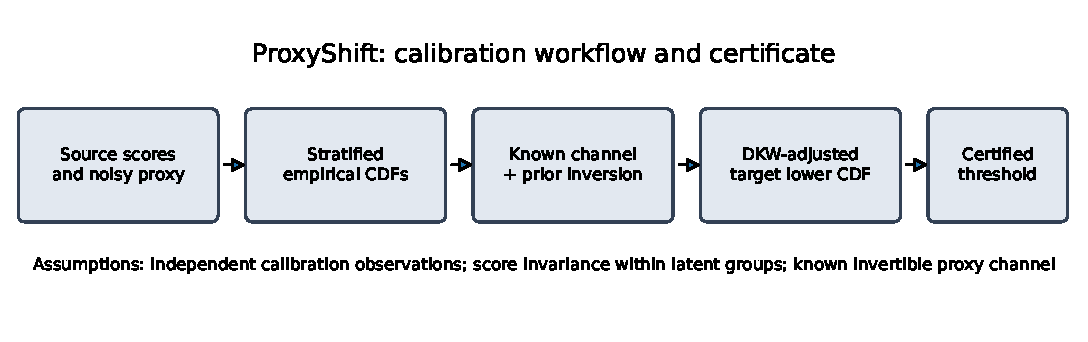
\includegraphics[width=\textwidth]{../figures/method_flowchart.pdf}
\caption{Calibration workflow. A known, invertible proxy channel and source mixture are necessary inputs, not quantities inferred from noisy scores alone. The output is a global score threshold or $+\infty$.}\label{fig:method}
\end{figure}

\section{A Finite-Sample Coverage Certificate}
Within the observed proxy stratum $z$, let $n_z=\#\{i:Z_i=z\}$ and
\[ \widehat F_z^Z(t)= n_z^{-1}\sum_{i:Z_i=z}\mathbf 1\{S_i\leq t\}\qquad (n_z>0).\]
For $n_z=0$ set $\widehat F_z^Z(t)=0$ and $\varepsilon_z=1$. For $n_z>0$, define
\begin{equation}\label{eq:epsilon}
 \varepsilon_z=\min\left\{1,\sqrt{\frac{\log(2K/\delta)}{2n_z}}\right\}, \quad 0<\delta<1.
\end{equation}
The two-sided Dvoretzky--Kiefer--Wolfowitz--Massart inequality \citep{massart1990} holds conditionally on the observed stratum sizes, because within each proxy stratum the scores are independently drawn from its conditional distribution. Define the estimated shifted CDF and an error allowance,
\begin{equation}\label{eq:bound}
 \widehat F_\tau(t)=\sum_z b_z(\tau)p_z\widehat F_z^Z(t),\qquad
 B_\tau=\sum_z|b_z(\tau)|p_z\varepsilon_z,\qquad
 L_\tau(t)=\widehat F_\tau(t)-B_\tau.
\end{equation}
No monotonicity is claimed for $\widehat F_\tau$, because negative inversion coefficients can induce small downward jumps.

\begin{theorem}[Simultaneous target coverage certificate]\label{thm:cert}
Under the four assumptions above, with calibration probability at least $1-\delta$, simultaneously for every real $t$ and every target mixture $\tau\in\mathcal T$,
\[F_\tau(t)\ge L_\tau(t).\]
Consequently, let $\widehat q$ be any finite calibration-data-measurable threshold such that
\begin{equation}\label{eq:choice}
 \inf_{\tau\in\mathcal T}L_\tau(\widehat q)\ge1-\alpha.
\end{equation}
Then, with calibration probability at least $1-\delta$, an independent target observation satisfies $\PR_Q\{S_{\mathrm{test}}\le \widehat q\mid \mathcal D_{\mathrm{cal}}\}\ge1-\alpha$ for every $\tau\in\mathcal T$. If no finite threshold satisfies \eqref{eq:choice}, choosing $\widehat q=+\infty$ preserves coverage, but produces a vacuous prediction region.
\end{theorem}
\begin{proof}
Conditional on $(n_1,\ldots,n_K)$, the DKW--Massart inequality and a union bound imply
$\PR(\sup_t|\widehat F_z^Z(t)-F_z^Z(t)|\le\varepsilon_z\ \forall z\mid n_1,\ldots,n_K)\ge1-\delta$.
On this event, for any $\tau$ and $t$, linearity of \eqref{eq:inversion} and the triangle inequality imply
$|\widehat F_\tau(t)-F_\tau(t)|\le\sum_z|b_z(\tau)|p_z\varepsilon_z=B_\tau$.
The DKW event holds simultaneously in $t$ and does not depend on $\tau$, so it also holds if $\tau$ or $\widehat q$ are chosen after calibration. At a threshold satisfying \eqref{eq:choice}, $F_\tau(\widehat q)\ge1-\alpha$ for every allowed target. The infinite threshold gives coverage one by definition. Averaging the conditional probability over the stratum counts completes the result.
\end{proof}

The theorem's guarantee is explicitly \emph{high-probability conditional coverage}, not an exact $1-\alpha$ unconditional split-conformal guarantee. A direct implication is unconditional coverage at least $(1-\delta)(1-\alpha)$ for a fixed admissible target. To require unconditional target coverage at least $1-\alpha_0$ from this argument, choose the internal nominal level $1-\alpha=(1-\alpha_0)/(1-\delta)$, where $\delta<\alpha_0$. This uses a more conservative threshold and is not the level used in the experiment below. Failure to distinguish the two guarantees would overstate the method.

\begin{corollary}[Sufficient condition for a finite threshold]\label{cor:finite}
For finite calibration scores with all proxy strata populated ($n_z>0$), $\mathcal T=\{\tau\}$, and $\varepsilon_z$ defined by \eqref{eq:epsilon}, the condition $B_\tau\le\alpha$ is sufficient for a finite threshold satisfying \eqref{eq:choice} to exist.
\end{corollary}
\begin{proof}
The inversion identity implies $\sum_zb_z(\tau)p_z=1$. At the maximum observed score, each empirical proxy-stratum CDF equals one provided that its stratum is populated. Thus $\widehat F_\tau(\max_i S_i)=1$ when all proxy strata are populated, and the corresponding lower bound is $1-B_\tau$. It reaches the requested $1-\alpha$ level whenever $B_\tau\le\alpha$. When some stratum is empty, the algorithm instead invokes its explicit conservative empty-stratum rule, and finite-threshold feasibility must be checked directly.
\end{proof}

\noindent This distinction matters in implementation: no proof relies on a signed empirical CDF being monotone. The algorithm searches all observed score values and selects the first certified threshold if one exists. In many noisy-proxy settings $B_\tau>\alpha$ and the procedure returns $+\infty$, as observed in the experiments.

\begin{proposition}[Robustness to within-group score drift]\label{prop:drift}
Suppose the score laws in the target have group-conditional CDFs $F_g^Q$ obeying $\sup_t|F_g^Q(t)-F_g^P(t)|\le\gamma_g$. On the same calibration event as Theorem~\ref{thm:cert}, for every $\tau$ and $t$,
\[F_\tau^Q(t)\ge L_\tau(t)-\sum_g\tau_g\gamma_g.\]
\end{proposition}
\begin{proof}
Apply the triangle inequality to $\sum_g\tau_g(F_g^Q(t)-F_g^P(t))$, then combine with Theorem~\ref{thm:cert}.
\end{proof}
If the $\gamma_g$ are unknown, this proposition is only a sensitivity identity, not a practically certifiable robustness result.

\section{Identifiability and the Price of Proxy Noise}
A nonsingular error channel is not a cosmetic assumption. Consider two equally probable latent groups with score distributions concentrated at $0$ and $1$. Let the proxy be independent of the latent group, so the two columns of $M$ coincide. Interchanging the two latent score laws leaves the observable source distribution of $(S,Z)$ unchanged. Under a target mixture assigning probability $0.8$ to the second group, however, the target CDF below score $1$ changes from $0.2$ to $0.8$. No procedure using only source $(S,Z)$ and this singular channel can uniquely recover target coverage. This elementary construction makes the identification boundary concrete.

For the two-group symmetric flip channel $M_\eta=\left(\begin{smallmatrix}1-\eta&\eta\\\eta&1-\eta\end{smallmatrix}\right)$, the determinant is $1-2\eta$. The inverse coefficients grow as $\eta$ approaches $1/2$, unless source and target mixtures align in a way that cancels the unstable direction. Consequently $B_\tau$ can grow substantially even when sample size is fixed. This is an honest signal that the available labels lack the information needed for a narrow certified interval.

\section{Computation and Complexity}
Figure~\ref{fig:method} summarizes the workflow. With $n$ scores and $K$ proxy states, we compute $b(\tau)$ by solving $A^\top b=\tau$, sort scores within each stratum and the pooled sample, and evaluate each empirical CDF on the pooled score grid. A straightforward implementation takes $O(Kn\log n+K^3)$ time and $O(Kn)$ temporary storage; for small $K$ it is dominated by sorting. A direct inversion of $A$ is unnecessary in software and is avoided in favor of a linear solve.

For a finite set of target mixtures, require all their lower bounds to cross the desired threshold. For $K=2$ and a convex interval of target mixture proportions, $L_\tau(t)$ in \eqref{eq:bound} is not necessarily affine in $\tau$ because of the absolute-value penalty. It is concave in $\tau$ (an affine estimator minus a convex norm), so its minimum over a closed line segment occurs at an endpoint. Thus checking both endpoint mixtures suffices for robust certification over an entire interval. The same argument extends to vertices of a compact polytope in higher dimensions. This yields a computationally small distributionally robust extension without an optimization search over all mixtures.

\section{Experiments}
\subsection{Design and Reproducibility}
We fix the calibration target $\alpha=0.1$ and confidence failure probability $\delta=0.1$. In each independent Monte Carlo repetition, the calibration population contains group B with probability $0.2$, while the target share is varied among $0.2$, $0.5$, and $0.8$. Group A scores follow $|N(0,1)|$, and group B scores follow $|N(0,3^2)|$. The proxy flips a group label symmetrically with probabilities $0.05$, $0.15$, $0.25$, or $0.40$, independently of scores conditional on group. We use $16{,}000$ calibration samples and $10{,}000$ independently generated target samples in each repetition, with 35 repetitions for each noise level. The source mixture and channel are supplied to the algorithm as ground truth; this deliberately tests identification and sampling error rather than the error from estimating the channel.

Baselines are (i) pooled split conformal; (ii) the signed inversion plug-in without the finite-sample penalty; and (iii) a \emph{diagnostic oracle} that sees true calibration group labels and estimates the mixture-specific target CDF directly. The oracle is not a deployable method under our data restrictions and is included only as a reference for the information cost of noisy proxies. Thresholds are evaluated using held-out coverage; for absolute residuals, interval half-width equals the chosen threshold. All CSV records, scripts, fixed seeds, and plotted figures are included in the reproducibility package.

\subsection{Shift and Coverage}
Table~\ref{tab:main} reports the most difficult non-vacuous primary setting, proxy flip probability $0.15$ and target group-B share $0.8$. Pooled calibration substantially undercovers (mean $0.655$). Both the uncorrected proxy inversion and the oracle approach $0.90$ empirically, but only the conservative method supplies the finite-sample conditional confidence statement proved here. It attains mean observed coverage $0.935$, at the cost of a longer half-width than the oracle. These are Monte Carlo outcomes in an explicit Gaussian model, not a claim of state-of-the-art performance on a real data benchmark.
\begin{table}[t]
\centering\small\begin{tabular}{lrrrr}
\hline
Calibration rule & Coverage & SD & Half-width & Vacuous \\
\hline
Pooled split conformal & 0.655 & 0.005 & 2.379 & 0.0\% \\
Uncorrected proxy inversion & 0.903 & 0.006 & 4.641 & 0.0\% \\
Latent-group oracle & 0.902 & 0.005 & 4.635 & 0.0\% \\
ProxyShift certificate & 0.935 & 0.004 & 5.233 & 0.0\% \\
\hline\end{tabular}

\caption{Main synthetic experiment: $n=16{,}000$, 35 repetitions, source B share $0.2$, target B share $0.8$, proxy error $0.15$. SD denotes across-repetition sample standard deviation of held-out coverage. Infinite widths are not present in this setting.}\label{tab:main}
\end{table}
\begin{figure}[t]
\centering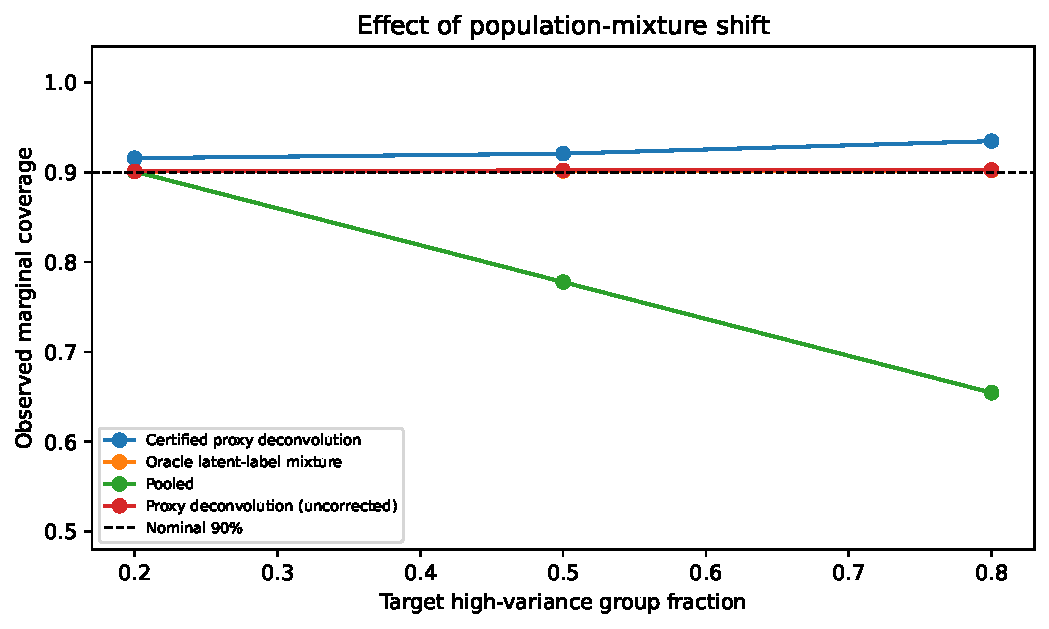
\includegraphics[width=.88\textwidth]{../figures/coverage_shift.pdf}
\caption{Marginal test coverage across target mixtures for proxy error probability $0.15$. The dashed line marks empirical $90\%$ nominal coverage. The certified method controls a distinct high-probability conditional objective.}\label{fig:coverage}
\end{figure}
\begin{figure}[t]
\centering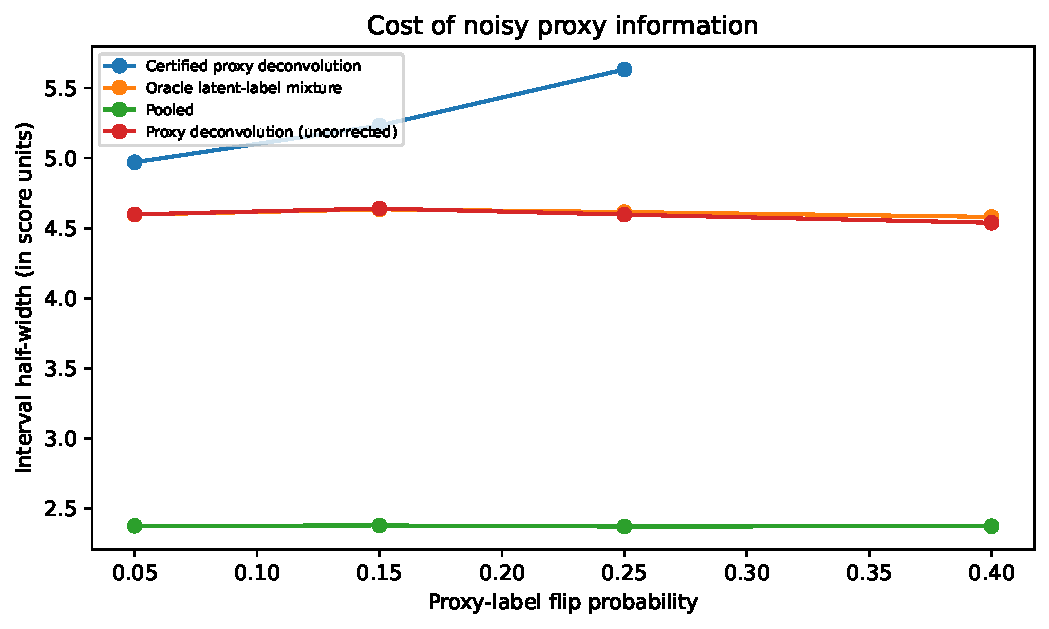
\includegraphics[width=.88\textwidth]{../figures/width_noise.pdf}
\caption{Half-widths versus proxy noise for target B share $0.8$. Missing finite points for the certified method indicate infinite prediction intervals, not zero width.}\label{fig:width}
\end{figure}
\begin{figure}[t]
\centering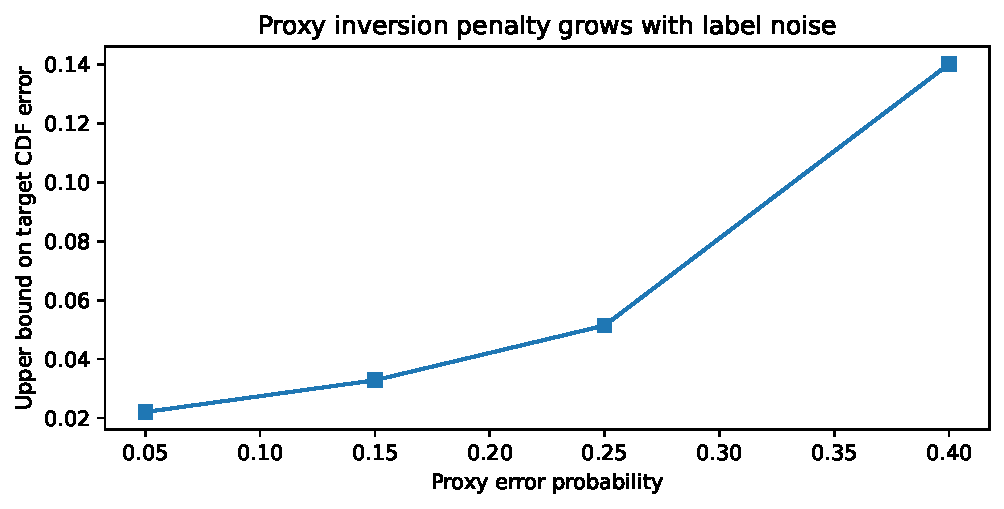
\includegraphics[width=.85\textwidth]{../figures/penalty_noise.pdf}
\caption{Mean DKW-based target-CDF correction $B_\tau$ as proxy quality degrades. The penalty reflects both sample sizes in the observed strata and amplification by signed inverse coefficients.}\label{fig:penalty}
\end{figure}

\subsection{When the Certificate Becomes Uninformative}
At target B share $0.8$ and proxy error $0.40$, the average uncertainty allowance is approximately $0.140$, exceeding the nominal miscoverage budget $0.10$. All 35 repetitions returned an infinite threshold. This is not a numerical error or an excluded outlier. The large inverse coefficients make a finite, high-confidence lower bound too weak in this regime. At proxy error $0.25$, the mean penalty falls to approximately $0.051$, and the certificate remains finite but tends to be conservative. These results are consistent with the inverse-channel conditioning argument in the preceding section.

\subsection{Exploratory Checks on Genuine Datasets}
To examine behavior outside the Gaussian model, we also used two standard public datasets packaged with scikit-learn \citep{pedregosa2011}: handwritten \emph{Digits} classification ($1{,}797$ examples) and \emph{Diabetes} regression ($442$ examples). Digits used a fixed multiclass logistic regression predictor with nonconformity score $1-\widehat p_y(x)$ and latent groups digits $0$--$4$ versus $5$--$9$. Diabetes used ridge regression and absolute residuals, with groups split by age relative to the training-split median. The proxy labels were synthetically corrupted at error probability $0.15$. We used 25 repeated train/calibration/test splits; source group proportions were set to observed calibration shares for this exploratory calculation and the test samples were reweighted within group to depict a hypothetical group-B fraction of $0.8$.

The results in Table~\ref{tab:real} should be interpreted cautiously. With only about 134 calibration points in Diabetes, the certificate is vacuous in every split. In Digits, with about 543 calibration points, the certificate is finite but covers approximately $98.3\%$ in this experiment and is much wider than the oracle. These are not formal validation of the theorem on an unknown deployment population: finite datasets, estimated source proportions and constructed shifts do not satisfy every known-population assumption exactly. They nevertheless demonstrate an important practical cost of the method that simulation with $n=16{,}000$ might conceal.
\begin{table}[t]
\centering\small\begin{tabular}{llrr}
\hline
Dataset & Calibration rule & Coverage & Vacuous \\
\hline
Digits & Pooled & 0.896 & 0\% \\
Digits & Uncorrected & 0.903 & 0\% \\
Digits & Certified & 0.983 & 0\% \\
Diabetes & Pooled & 0.904 & 0\% \\
Diabetes & Uncorrected & 0.890 & 0\% \\
Diabetes & Certified & 1.000 & 100\% \\
\hline\end{tabular}

\caption{Exploratory real-dataset checks at hypothetical target group-B share $0.8$, 25 repeated splits, proxy error $0.15$. Vacuous means $q=+\infty$, for which the displayed empirical coverage is one. Source proportions are estimated in this illustration and thus are outside the exact known-prior theorem.}\label{tab:real}
\end{table}

\subsection{Controlled Real-Data Score-Population Experiment}
A second benchmark separates the assumptions of the theorem from a generalization claim about real deployments. We fit logistic-regression classifiers on the \texttt{Digits}, \texttt{Wine}, and \texttt{Breast Cancer} data sets and a ridge-regression model on \texttt{Diabetes} (all accessed through scikit-learn). We reserve 45\% of each data set for fitting. The remaining 55\% supplies two \emph{fixed empirical distributions} of nonconformity scores, indexed by the binary group. Digits uses labels below five versus at least five; Wine uses class two versus the other classes; Breast Cancer uses its two outcome labels. The Diabetes group is defined by the median of the age-related input variable measured in the training partition. The training data are excluded from the score-population pool.

Conditional on the trained predictor and each empirical pool, \emph{every} calibration and evaluation score is independently sampled \emph{with replacement} from its group's fixed score distribution. In particular, the source group probabilities $(0.8,0.2)$, the target group probabilities $(0.2,0.8)$, and a symmetric proxy-flip channel with error 0.15 are design parameters \emph{known exactly} to the algorithms. This finite-support experiment therefore satisfies the within-group stability and known-parameter conditions of Theorem~\ref{thm:cert} conditional on the fixed empirical pools. It is a controlled stress test built from genuine prediction errors---\emph{not} an estimate of out-of-sample performance on independent patients, users, or institutions. Reusing some underlying held-out score values across sampling repetitions is inherent to the with-replacement protocol; the draws, rather than the finite original examples, are independent conditional on the fixed pools.

With $16{,}000$ calibration draws, $10{,}000$ evaluation draws, and 30 replicates, Table~\ref{tab:empirical} compares pooled calibration, signed inversion without a confidence penalty, the certified proxy method, and two oracles that observe true latent group labels. One oracle estimates the target CDF directly, while the second applies the same DKW certification method with an identity observation channel; neither oracle is deployable when only proxies are recorded. The empirical conditional coverages are also computed analytically from the finite empirical score distributions, without test-sample Monte Carlo error. Repetitions varied calibration draws and proxy noise, \emph{not} the underlying fitted model or empirical population. Accordingly, reported means and uncertainty across these repetitions describe calibration randomness alone.

\begin{table}[t]
\centering\small\begin{tabular}{llrr}
\hline
Data set & Method & Coverage & Mean half-width \\
\hline
Digits & Pooled & 0.884 & 0.214 \\
 & Proxy plug-in & 0.902 & 0.257 \\
 & Proxy certificate & 0.935 & 0.447 \\
 & Latent oracle + DKW & 0.923 & 0.366 \\
\hline
Diabetes & Pooled & 0.907 & 93.385 \\
 & Proxy plug-in & 0.903 & 91.032 \\
 & Proxy certificate & 0.935 & 106.405 \\
 & Latent oracle + DKW & 0.925 & 101.646 \\
\hline
Wine & Pooled & 0.944 & 0.196 \\
 & Proxy plug-in & 0.921 & 0.111 \\
 & Proxy certificate & 0.937 & 0.143 \\
 & Latent oracle + DKW & 0.931 & 0.112 \\
\hline
Breast Cancer & Pooled & 0.966 & 0.200 \\
 & Proxy plug-in & 0.901 & 0.078 \\
 & Proxy certificate & 0.935 & 0.101 \\
 & Latent oracle + DKW & 0.923 & 0.089 \\
\hline
\end{tabular}

\caption{Known-prior empirical-population benchmark, 30 independent calibration replications, 16,000 calibration and 10,000 evaluation draws per replication. Coverage is held-out containment frequency. No certified interval was vacuous in these four controlled settings; full data and exact group-conditional population CDF checks appear in the repository.}
\label{tab:empirical}
\end{table}

\begin{figure}[t]
\centering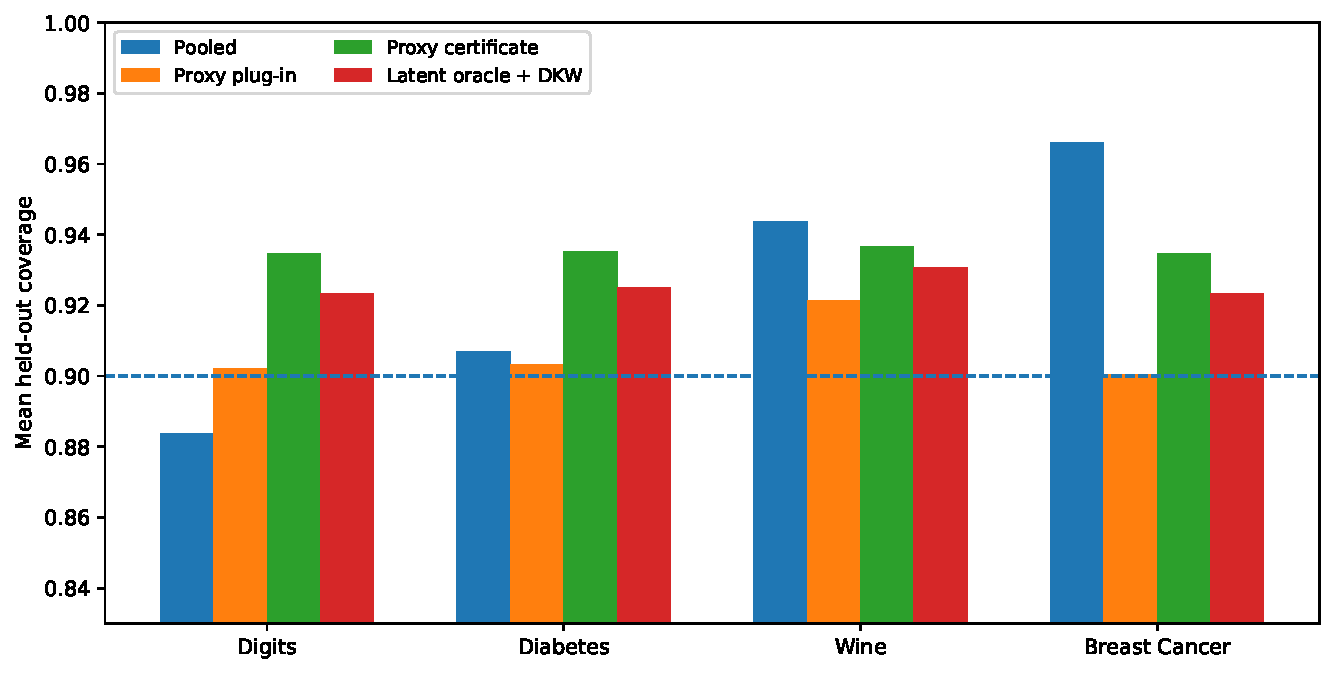
\includegraphics[width=.88\textwidth]{../figures/known_prior_comparison.pdf}
\caption{Mean coverage across controlled finite-population resampling studies. The horizontal line marks the 90\% target; values are empirical coverage, not the finite-sample conditional guarantee itself.}
\label{fig:knownprior}
\end{figure}

The main pattern is informative but qualified: the proxy certificate attains 93--94\% average coverage across these constructed mixtures, at a cost in threshold width relative to the latent-label oracles. Pooled calibration behaves differently across populations: it undercovers in Digits but is conservative in Breast Cancer and Wine. This heterogeneity cautions against drawing conclusions about deployment from the Gaussian example alone. The conditionally fixed empirical populations create a theory-matched setting, but they do not address misspecification of $M$, $\pi$ or $\tau$, drift within latent groups, or generalization beyond the finite score support.

\section{Discussion}
Three lessons emerge. First, subgroup mixture changes can invalidate a pooled calibration threshold even when the conditional distribution of the score within each true group stays fixed. Second, noisy group labels create an identification problem rather than just a modest variance increase: if the channel is well-conditioned and known, inverse mixtures can recover the target score CDF; as it approaches singularity, the bound becomes weak or vacuous. Third, high-probability conditional certification is not free. The method is conservative, particularly for small samples, and it often cannot produce a practically useful interval.

A major unresolved issue is obtaining the source group proportions, the target mixture, and the proxy channel independently of the calibration data. Plug-in estimates of these inputs do not automatically inherit Theorem~\ref{thm:cert}. A proper extension would use independent validation data to construct a confidence region for $(M,\pi,\tau)$ and minimize the lower envelope over that region. The paper does not implement or claim that extension.

Several limitations further constrain interpretation. The conditional-independence assumption may fail when large residuals cause more proxy mistakes. The target score distribution can drift within group, rather than changing only by mixture, in which case Proposition~\ref{prop:drift} requires independently justified drift bounds. The theorem certifies a global interval and does not establish group-conditional coverage or efficiency optimality. The experiments remain limited in breadth: the Gaussian generator has two residual scales, ordinary train/calibration splits show strong conservatism, and the controlled four-data-set resampling study only examines fixed empirical score distributions. Although the latter obeys the theorem's assumptions by design, it is not an independent field evaluation. Comparisons with fully implemented recent published methods and independent novelty assessment remain necessary before any claim of a broadly impactful methodological advance.

\section{Conclusion}
Noisy subgroup indicators do not automatically erase all information about shifted predictive coverage, but recovering that information requires assumptions about the error channel. We derived a score-distribution identity and a finite-sample confidence envelope that turn proxy-stratified calibration scores into a conservative target coverage certificate. The principal positive result is conditional reliability under a specified mixture-shift model; its principal negative result is the cost of that reliability, including infinite intervals when the proxy is too noisy or the sample too small. Reporting both is essential to understanding where the method can responsibly be used.

\acks{Generative AI tools assisted with literature triage, exploratory algorithm development, code implementation, drafting, and manuscript formatting. The named author remains responsible for checking the mathematical arguments, source references, experiment reproducibility, and submitted claims. Funding and competing-interest statements must be confirmed by the corresponding author as required by the journal before submission.}

\appendix
\section{Further Technical Notes}
\subsection{Vertex Reduction for Mixture Ambiguity}
For each fixed $t$, the function $\tau\mapsto\widehat F_\tau(t)$ is affine, while
$\tau\mapsto B_\tau=\sum_zp_z\varepsilon_z|\tau^\top A^{-1}e_z|$ is convex. Thus $L_\tau(t)$ is concave in $\tau$. If $\mathcal T$ is the convex hull of a finite set of vertices $V$, then for any convex combination $\tau=\sum_{v\in V}\lambda_v v$,
\[L_\tau(t)\ge\sum_{v\in V}\lambda_vL_v(t)\ge\min_{v\in V}L_v(t).\]
Therefore checking only vertices is sufficient and necessary for the worst-case lower-envelope condition.

\subsection{Analytical Target Score CDF for the Gaussian Experiment}
In the simulation, for nonnegative $t$ and target group-B share $\rho$, the true score CDF is
\[ F_\rho(t)=(1-\rho)\,\operatorname{erf}\!\left(\frac{t}{\sqrt 2}\right)+\rho\,\operatorname{erf}\!\left(\frac{t}{3\sqrt2}\right).\]
This expression gives an independent population-level check on each threshold without relying exclusively on finite target test sets. The experimental script reports held-out empirical coverage; a separate assertion can evaluate the formula at every finite threshold. Conditional population coverage is not itself estimated by pooling all Monte Carlo test observations under one random threshold.

\subsection{Reproducibility Details}
The accompanying source archive includes the random seeds, exact dependency requirements, individual trial records, aggregate tables, and original figure data. To rebuild the results from the project root, run \path{src/experiment.py} for the Gaussian study; \path{src/real_data.py} for the exploratory ordinary splits; and \path{src/known_prior_benchmark.py} for the theory-matched empirical score populations. Regenerate tables using \path{src/generate_tables.py}; the newest table and figure are also included in the package. Tests are available under \path{tests/}. No claim is made about human participants, external clinical validity, live deployment, or superiority over unimplemented published baselines.

\bibliographystyle{plainnat}
\begin{thebibliography}{12}
\bibitem[Angelopoulos and Bates(2023)]{angelopoulos2023} Anastasios N. Angelopoulos and Stephen Bates. Conformal prediction: A gentle introduction. \emph{Foundations and Trends in Machine Learning}, 16(4):494--591, 2023. doi:10.1561/2200000101.
\bibitem[Bhattacharyya and Barber(2026)]{bhattacharyya2026} Aabesh Bhattacharyya and Rina Foygel Barber. Group-weighted conformal prediction. \emph{Electronic Journal of Statistics}, 20(1), 2026. doi:10.1214/26-EJS2506.
\bibitem[Feldman et~al.(2026)]{feldman2026} Shai Feldman, Stephen Bates, and Yaniv Romano. Conformal prediction with corrupted labels: Uncertain imputation and robust re-weighting. In \emph{International Conference on Learning Representations}, 2026.
\bibitem[Gibbs et~al.(2025)]{gibbs2025} Isaac Gibbs, John J. Cherian, and Emmanuel J. Cand\`es. Conformal prediction with conditional guarantees. \emph{Journal of the Royal Statistical Society: Series B}, 87(4):1100--1126, 2025. doi:10.1093/jrsssb/qkaf008.
\bibitem[Lipton et~al.(2018)]{lipton2018} Zachary C. Lipton, Yu-Xiang Wang, and Alexander J. Smola. Detecting and correcting for label shift with black box predictors. In \emph{Proceedings of the 35th International Conference on Machine Learning}, Proceedings of Machine Learning Research, 80:3122--3130, 2018.
\bibitem[Massart(1990)]{massart1990} Pascal Massart. The tight constant in the Dvoretzky--Kiefer--Wolfowitz inequality. \emph{The Annals of Probability}, 18(3):1269--1283, 1990.
\bibitem[Pedregosa et~al.(2011)]{pedregosa2011} Fabian Pedregosa et al. Scikit-learn: Machine learning in Python. \emph{Journal of Machine Learning Research}, 12:2825--2830, 2011.
\bibitem[Podkopaev and Ramdas(2021)]{podkopaev2021} Aleksandr Podkopaev and Aaditya Ramdas. Distribution-free uncertainty quantification for classification under label shift. \emph{Proceedings of Machine Learning Research}, 161:844--853, 2021.
\bibitem[Sesia et~al.(2025)]{sesia2025} Matteo Sesia et al. Adaptive conformal classification with noisy labels. \emph{Journal of the Royal Statistical Society: Series B}, 87(3):796--815, 2025. doi:10.1093/jrsssb/qkae114.
\bibitem[Tibshirani et~al.(2019)]{tibshirani2019} Ryan J. Tibshirani, Rina Foygel Barber, Emmanuel J. Cand\`es, and Aaditya Ramdas. Conformal prediction under covariate shift. \emph{Advances in Neural Information Processing Systems}, 32, 2019.
\bibitem[Vovk et~al.(2005)]{vovk2005} Vladimir Vovk, Alexander Gammerman, and Glenn Shafer. \emph{Algorithmic Learning in a Random World}. Springer, 2005.
\bibitem[Yang and Jin(2026)]{yang2026} Yuqi Yang and Ying Jin. Multi-distribution robust conformal prediction. In \emph{Proceedings of the 43rd International Conference on Machine Learning}, Proceedings of Machine Learning Research, volume 306, pages 144952--145007, 2026.
\end{thebibliography}
\end{document}